\documentclass{beamer}
\usetheme{Boadilla}
\usefonttheme{serif}
%\usepackage{amscd}
\usepackage{amsmath}
\usepackage[makeroom]{cancel}
\usepackage{verbatim}
%\usepackage{amssymb}

\title{Gmacs}
\subtitle{A generalized size-structured stock assessment model}
\author{The Gmacs Development Team}
%\institute{Quantifish}
\date{\today}
\begin{document}

%% =========================================================================== %%

\begin{frame}
\titlepage
\end{frame}

%% =========================================================================== %%

\begin{frame}
\frametitle{Outline}
\tableofcontents
\end{frame}

%% =========================================================================== %%
%% =========================================================================== %%

\section{Notation and some definitions}

%% =========================================================================== %%
%% =========================================================================== %%

\subsection{Notation}
\begin{frame}
\frametitle{Notation}
Generally
\begin{itemize}
\item a bold capital symbol ${\bf A}$ refers to a matrix
\item a bold lowercase symbol ${\bf a}$ refers to a vector
\item an unbolded italic symbol $a$ refers to a scalar
\item $\{ a_i \}^n_{i=1}$ is an ordered $n$-tuple
\item the terms $p(\cdot)$ or $\pi(\cdot)$ represent probability
  distributions
\item $a|b$ means event $a$ conditional on event $b$ having occurred
\item the symbol $\forall$ means for all values, usually referring to all of the
  values within an ordered tuple.
\end{itemize}
\end{frame}

%% =========================================================================== %%

\subsection{Indices}
\begin{frame}
\frametitle{Indices}
\begin{table}
  \centering
  \begin{tabular}{cl}
  \hline
  Symbol  & Description \\
  \hline
      $g$ & group \\
      $h$ & sex \\
      $i$ & year \\
      $j$ & time step (years) \\
      $k$ & gear or fleet \\
      $\ell$ & index for size class \\
      $m$ & index for maturity state \\
      $o$ & index for shell condition \\
  \hline
  \end{tabular}
\end{table}
Notice no area index.
\end{frame}

%% =========================================================================== %%

\subsection{Leading model parameters}
\begin{frame}
\frametitle{Leading model parameters}
\begin{table}
  \centering
  \begin{tabular}{ccl}
  \hline
  Symbol & Support & Description \\
  \hline
      \textcolor{red}{$M_0$} & $0 < \textcolor{red}{M_0} < \infty$ & Initial instantaneous natural mortality rate\\
      \textcolor{red}{$\bar{R}$} & $0 < \textcolor{red}{\bar{R}} < \infty$ & Average recruitment\\
      \textcolor{red}{$\ddot{R}$} & $\textcolor{red}{\ddot{R}} > 0$ &Initial recruitment\\
      \textcolor{red}{$\alpha_r$} & $\textcolor{red}{\alpha_r} > 0$ & Mode of size-at-recruitment\\
      \textcolor{red}{$\beta_r $} & $\textcolor{red}{\beta_r} > 0$ & Shape parameter for size-at-recruitment\\
      \textcolor{red}{$R_0$} & $\textcolor{red}{R_0} > 0$ & Unfished average recruitment\\
      \textcolor{red}{$\kappa$} & $\textcolor{red}{\kappa} > 1$ & Recruitment compensation ratio\\
  \hline
  \end{tabular}
\end{table}
We group the leading model parameters into the vector
\begin{equation*}
  \textcolor{red}{\boldsymbol\theta} = \{ \textcolor{red}{M_0},
  \textcolor{red}{\bar{R}}, 
  \textcolor{red}{\ddot{R}}, \textcolor{red}{\alpha_r},
  \textcolor{red}{\beta_r}, \textcolor{red}{R_0}, \textcolor{red}{\kappa} \}.
\end{equation*}
\end{frame}

%% =========================================================================== %%

\subsection{Growth parameters}
\begin{frame}
\frametitle{Growth parameters}
\begin{table}
  \centering
  \begin{tabular}{ccl}
  \hline
  Symbol & Support & Description \\
  \hline
      \textcolor{red}{$\alpha_h$} & $\textcolor{red}{\alpha_h} > 0$ & Mode of size-at-recruitment\\
      \textcolor{red}{$\beta_h$} & $\textcolor{red}{\beta_h} > 0$ & Shape parameter for size-at-recruitment\\
      \textcolor{red}{$\varphi_h$} & $\textcolor{red}{\varphi_h}$ & Instantaneous natural mortality rate\\
  \hline
  \end{tabular}
\end{table}
We group the growth parameters into the vector
\begin{equation*}
  \textcolor{red}{\boldsymbol\psi} = \{ \textcolor{red}{\alpha_h}, 
  \textcolor{red}{\beta_h}, \textcolor{red}{\varphi_h} \}.
\end{equation*}
\end{frame}

%% =========================================================================== %%

\subsection{Latent states}
\begin{frame}
\frametitle{Latent states}
\begin{table}
  \centering
  \begin{tabular}{ccl}
  \hline
  Symbol & Support & Description \\
  \hline
      \textcolor{red}{$\boldsymbol\nu$} & & Instantaneous natural mortality rate\\
      \textcolor{red}{$\boldsymbol\xi$} & &  Discard mortality rate\\
  \hline
  \end{tabular}
\end{table}
We group the latent states into the vector
\begin{equation*}
  \textcolor{red}{\boldsymbol\omega} = \{ \textcolor{red}{\boldsymbol\nu},
  \textcolor{red}{\boldsymbol\xi} \}.
\end{equation*}
\end{frame}

%% =========================================================================== %%

\subsection{Other variables}
\begin{frame}
\frametitle{Other variables}

\begin{table}
  \centering
  \begin{tabular}{ccl}
  \hline
  Symbol  & Dimensions & Description \\
  \hline
      $\boldsymbol{w}_{h}$ & $\ell \times 1$ & Mean weight at length ($\ell$) by sex ($h$) \\
      $\boldsymbol{m}_{h} $ & $\ell \times 1$ & Average proportion mature at length ($\ell$) by sex ($h$) \\
  \hline
  \end{tabular}
\end{table}

\begin{equation*}
  \boldsymbol{w}_{h} = f_w(\ell,\theta)
\end{equation*}

\begin{equation*}
  \boldsymbol{m}_{h} = f_m(\ell,\theta)
\end{equation*}


\end{frame}

%% =========================================================================== %%

\subsection{Cubic splines}
\begin{frame}
\frametitle{Cubic splines}
A spline is a numeric function that is piecewise-defined by polynomial
functions, and which possesses a sufficiently high degree of smoothness at the
places where the polynomial pieces connect (which are known as knots). A cubic
spline is constructed of piecewise third-order polynomials. The second
derivative of each polynomial is commonly set to zero at the endpoints, since
this provides a boundary condition that completes the system of $m-2$
equations. This produces a so-called ``natural'' cubic spline and leads to a
simple tridiagonal system which can be solved easily to give the coefficients of
the polynomials. However, this choice is not the only one possible, and other
boundary conditions can be used instead.
\end{frame}

%% =========================================================================== %%
%% =========================================================================== %%

\section{Growth}

%% =========================================================================== %%
%% =========================================================================== %%

\subsection{Growth}
\begin{frame}
\frametitle{Growth}
The average molt increment from size class $\ell$ to $\ell'$ is assumed to be
sex-specific and is defined by the linear function
\begin{equation*}
  a_{h,\ell} = \frac{\textcolor{red}{\alpha_h} + \textcolor{red}{\beta_h}
    \ell}{\textcolor{red}{\varphi_h}}.
\end{equation*}
The probability of transitioning from size class $\ell$ to $\ell'$ assumes that
variation in molt increments follows a gamma distribution
\begin{equation*}
  p (\ell'|\ell)_h = \boldsymbol{G}_h = \int^{\ell + \Delta \ell}_\ell \frac{\ell^{a_{h,\ell-1}} \exp
    \left(\frac{\ell}{\textcolor{red}{\varphi_h}} \right)}{\Gamma (a_{h,\ell}) \ell^{a_{h,\ell}}}
  \quad \text{where} \quad \Delta \ell = \ell' - \ell.
\end{equation*}
Specifically
\begin{equation*}
  \boldsymbol{G} = G_{\ell,\ell'} = \left( \begin{array}{cccc}
      G_{1,1} & G_{1,2} & \hdots & G_{1,n} \\
      G_{2,1} & G_{2,2} & \hdots & G_{2,n} \\
      \vdots & \vdots & \ddots & \vdots \\
      G_{n,1} & G_{n,2} & \hdots & G_{n,n} \end{array} \right)
  \quad \text{where} \quad \sum_{\ell'} G_{\ell,\ell'} = 1 \quad \forall \ell.
\end{equation*}
\end{frame}

%% =========================================================================== %%

\begin{frame}
\frametitle{Growth increment}
Growth increment
\begin{figure}[!htbp]
  \centering
  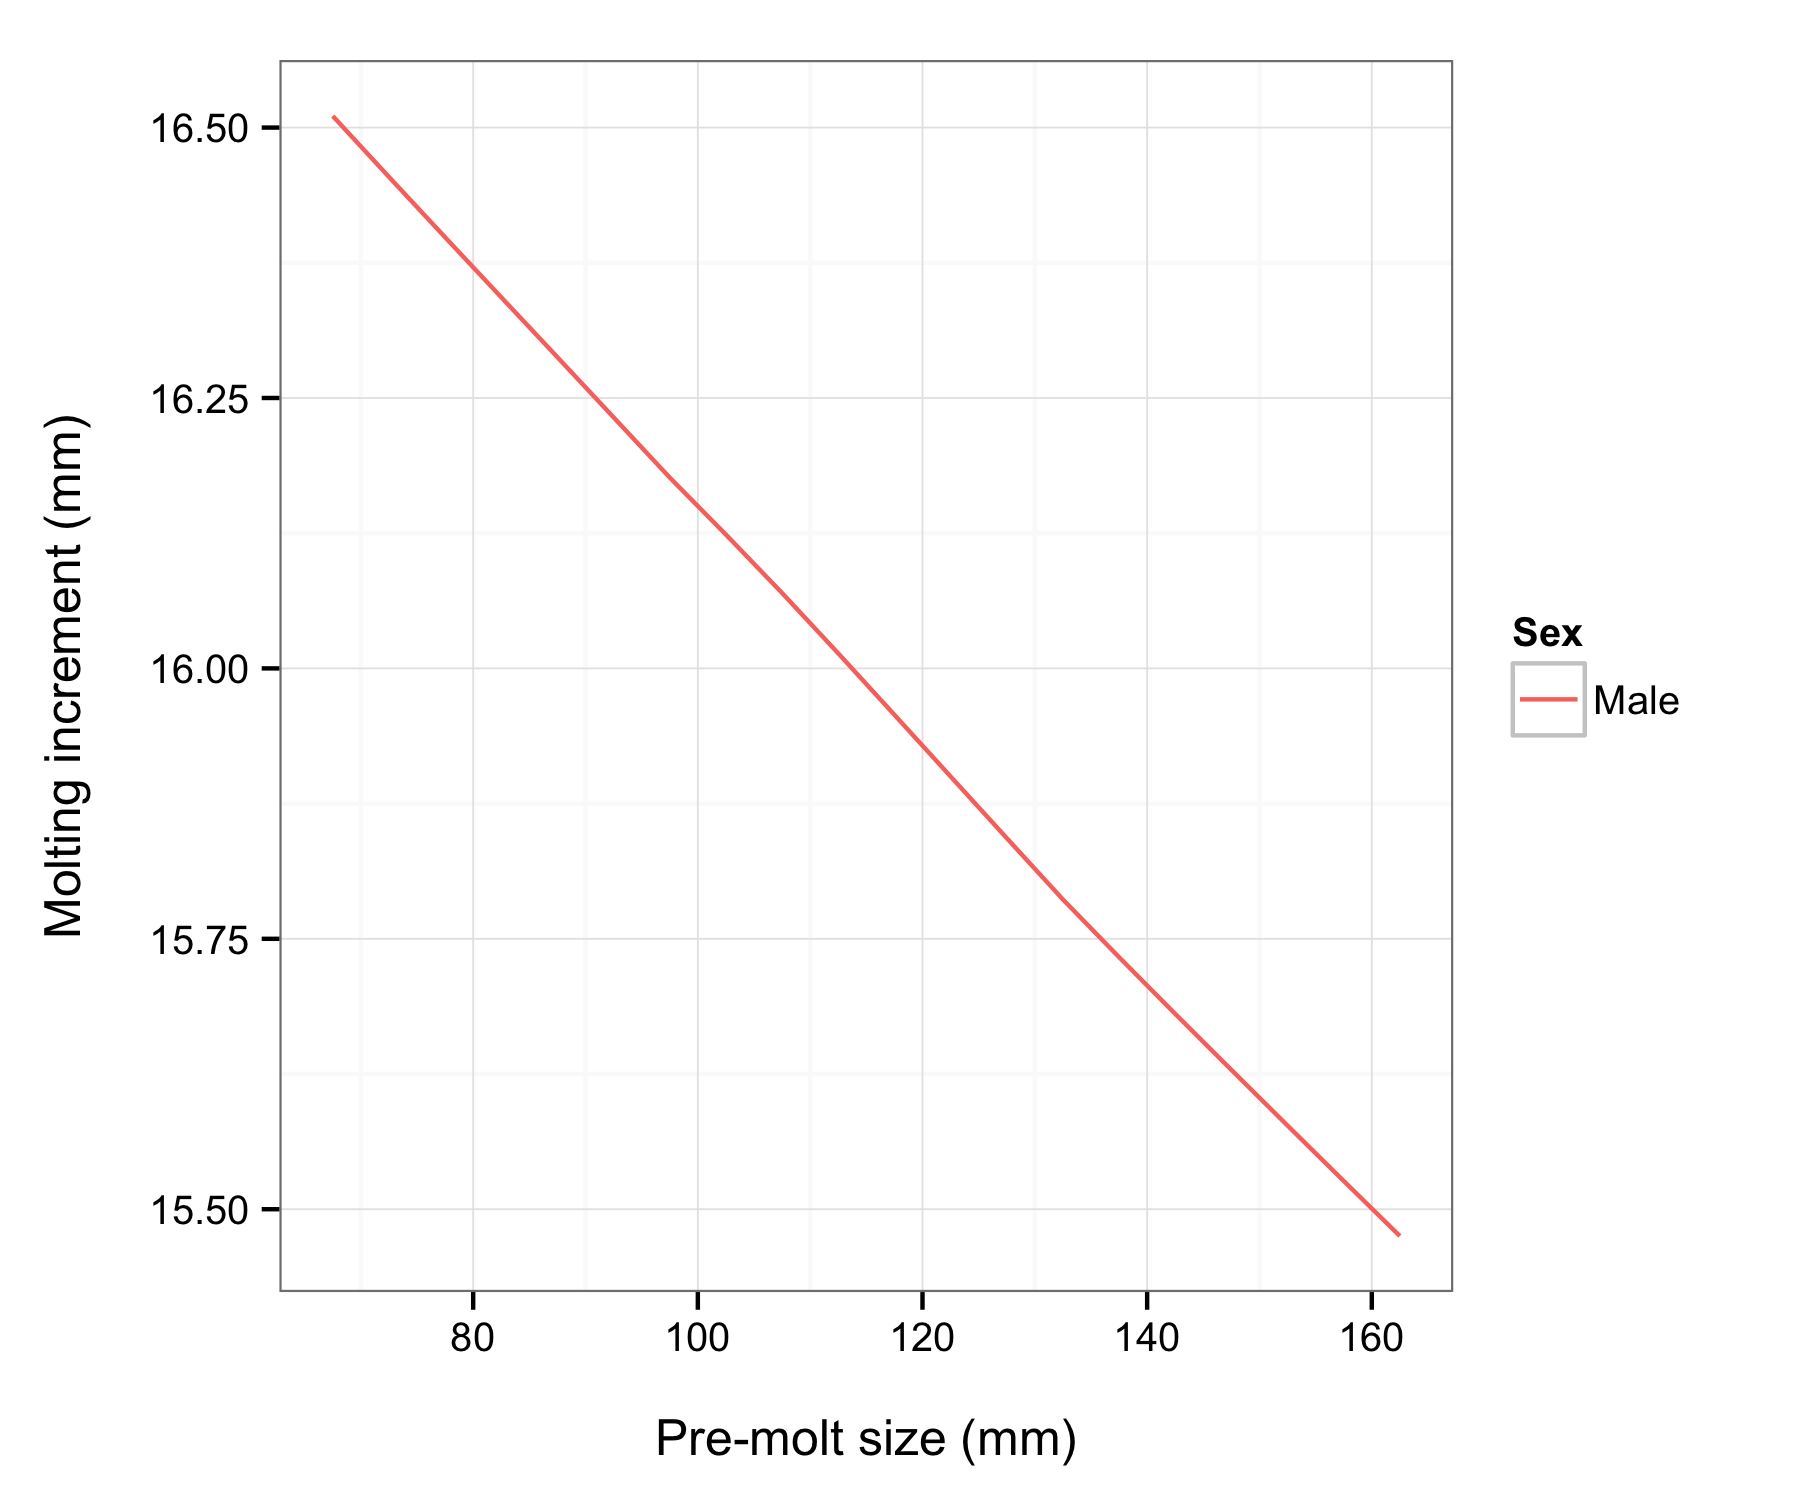
\includegraphics[width=0.75\linewidth]{../../examples/bbrkc/OneSex/figure/gi.png}
\end{figure}
\end{frame}

%% =========================================================================== %%

\begin{frame}
\frametitle{Growth}
Growth transition
\begin{figure}[!htbp]
  \centering
  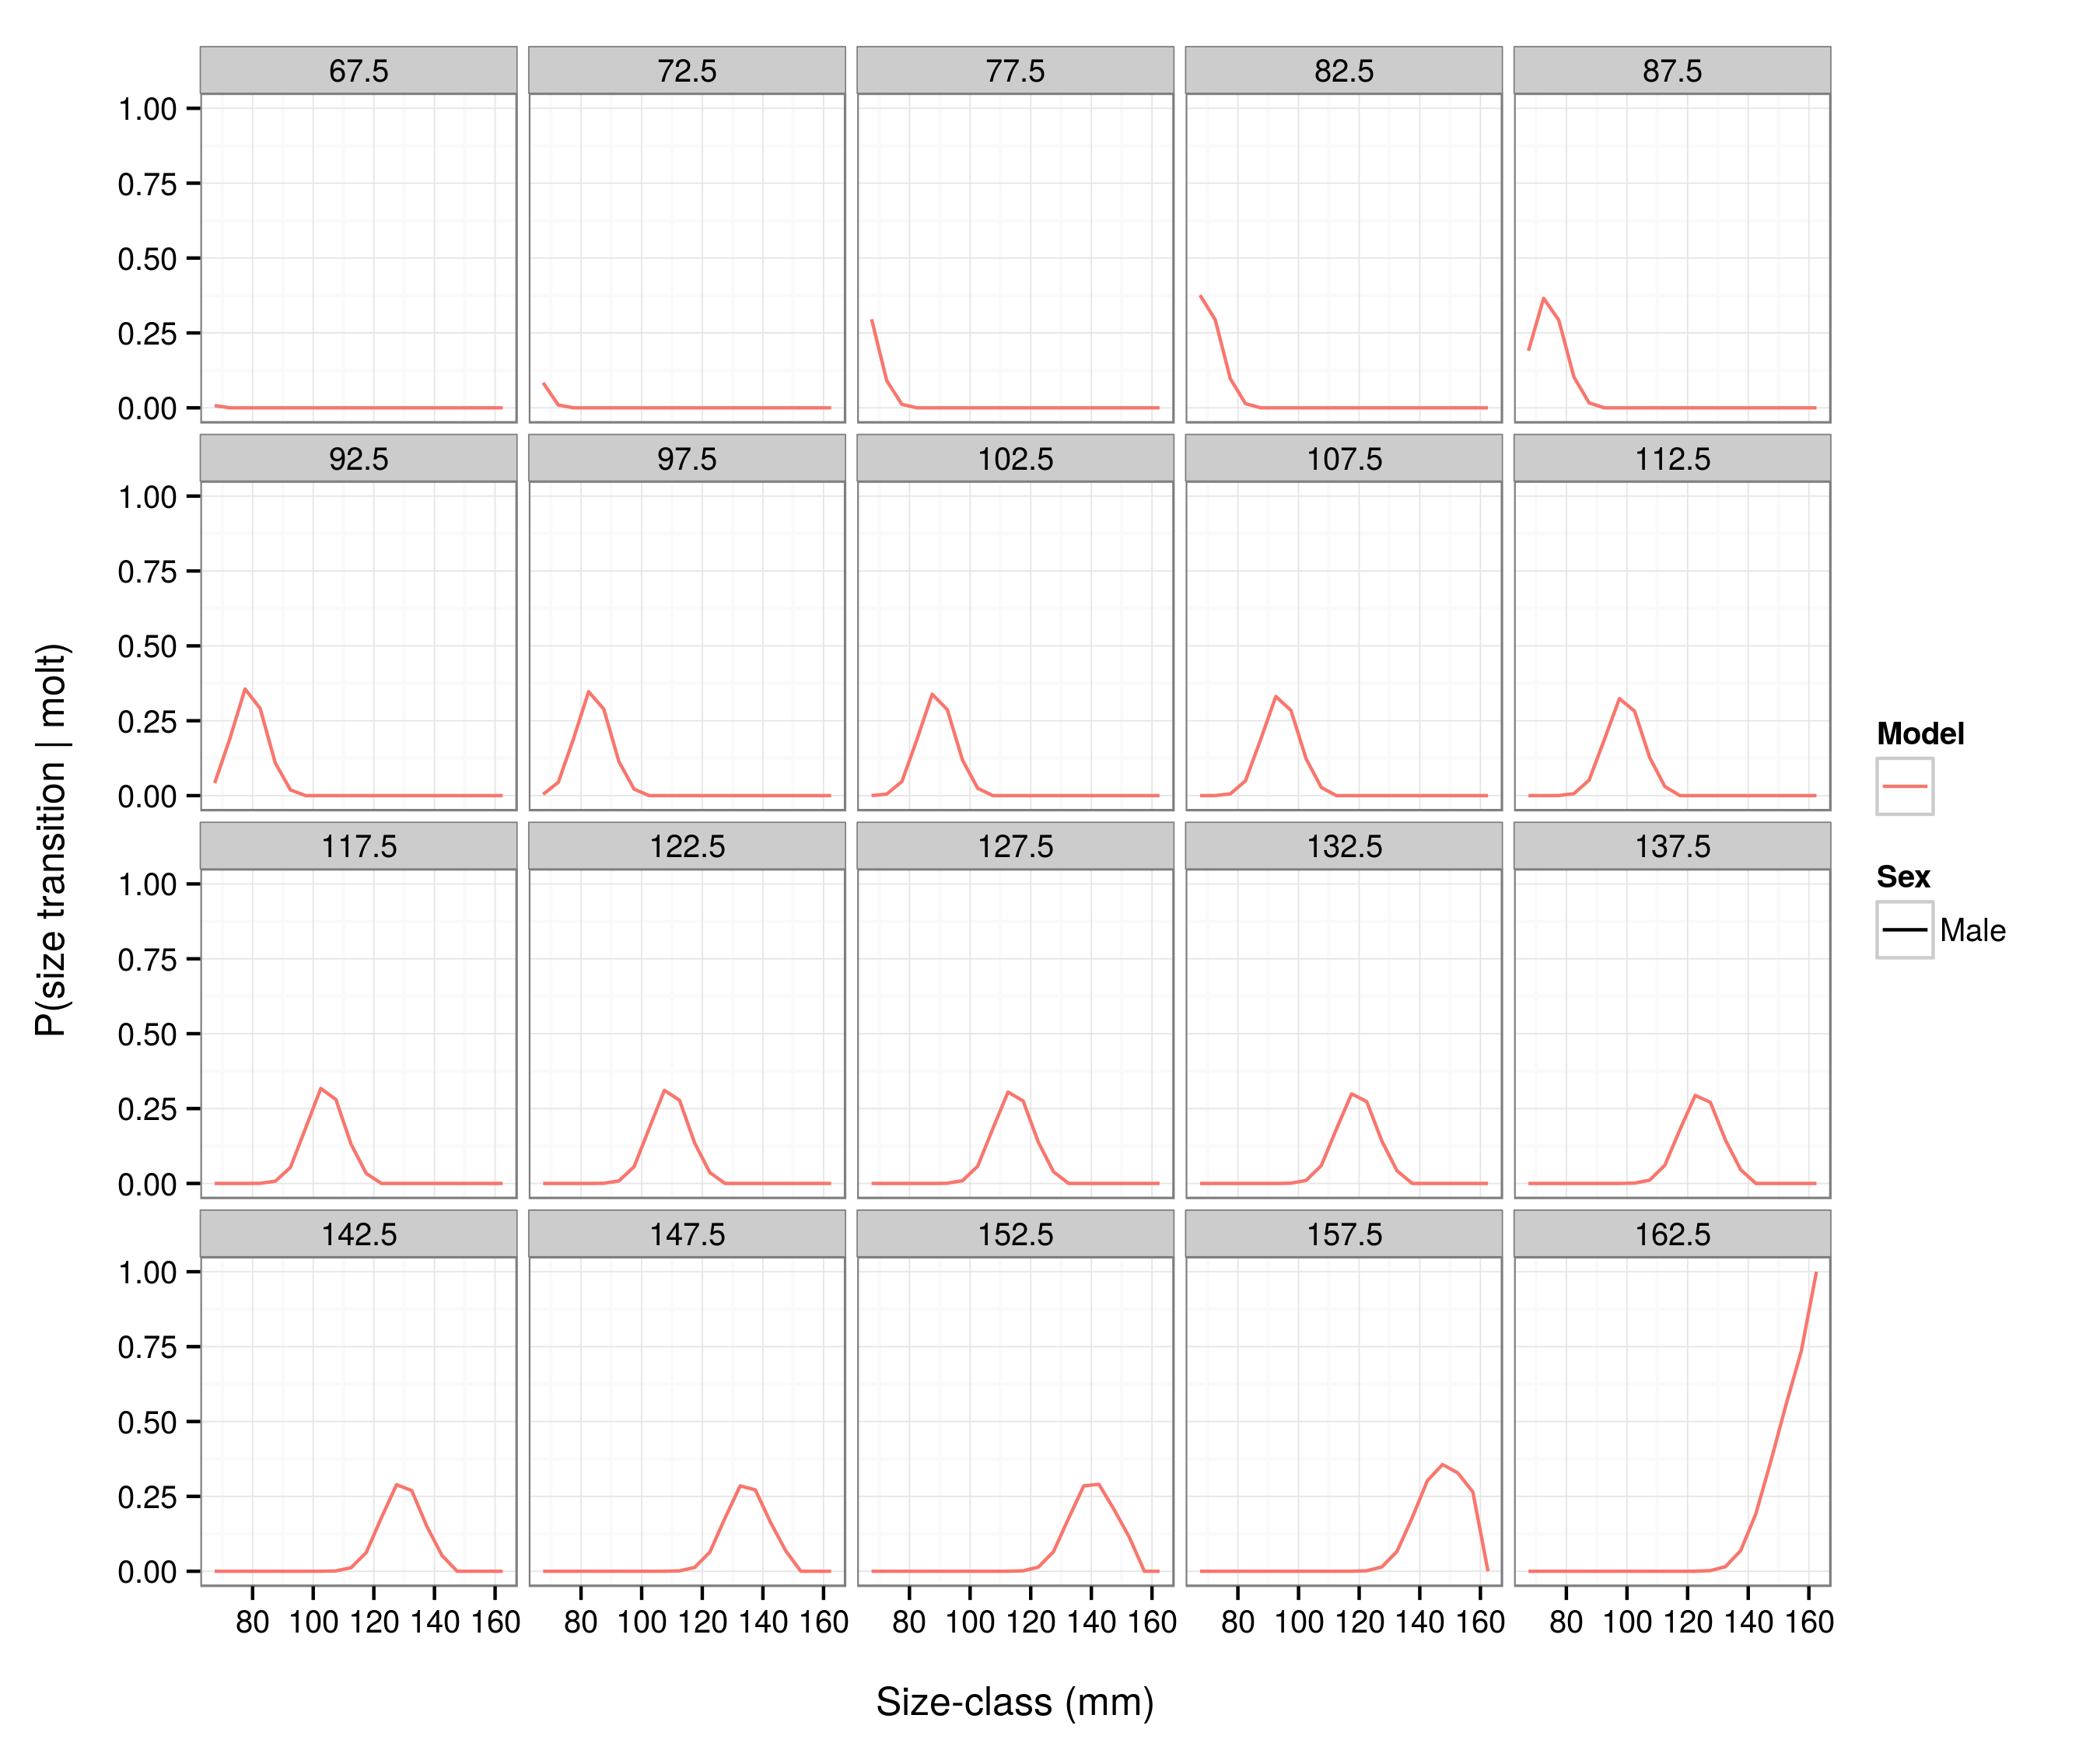
\includegraphics[width=0.75\linewidth]{../../examples/bbrkc/OneSex/figure/growth_transition.png}
\end{figure}
\end{frame}

%% =========================================================================== %%
%% =========================================================================== %%

\section{Selectivity, retention, fishing}

%% =========================================================================== %%
%% =========================================================================== %%

\subsection{Selectivity and retention}
\begin{frame}
\frametitle{Selectivity, retention and fishing mortality}
\begin{table}
  \centering
  \begin{tabular}{ccl}
  \hline
  Symbol & Dimensions & Description \\
  \hline
      \textcolor{red}{$a_{h,i,k}$} & $1$ & Length at 50\% selectivity \\
      \textcolor{red}{$\sigma^s_{h,i,k}$} & $1$ & Standard deviation in length at selectivity \\
      $\boldsymbol{s}_{h,i,k}$ & $\ell \times 1$ & Length at 50\% selectivity in length interval $\ell$ \\
      \textcolor{red}{$r_{h,i,k}$} & $1$ & Length at 50\% \\
      \textcolor{red}{$\sigma^y_{h,i,k}$} & $1$ & Standard deviation in length at retention \\
      $\boldsymbol{y}_{h,i,k}$ & $\ell \times 1$ & Length at 50\% retention in length interval $\ell$ \\
      \textcolor{red}{$\xi_{h,k}$} & $1$ & Discard mortality rate for sex $h$ and gear $k$ \\
      $\boldsymbol\nu_{h,i,k}$ & $\ell \times 1$ & Vulnerability due to fishing mortality for sex $h$ \\
      $\bar{\boldsymbol{f}}_k$ & $i \times 1$ & Average fishing mortality rate for gear $k$ \\
      $\boldsymbol\Psi_{k,i}$ & & Fishing mortality deviate for gear $k$ in year $i$ \\
      $\boldsymbol{F}_{k,i}$ & & Annual fishing mortality rate for gear $k$ in year $i$ \\
  \hline
  \end{tabular}
\end{table}
\end{frame}

%% =========================================================================== %%

\begin{frame}
\frametitle{Selectivity and retention}
The probability of catching an animal of sex $h$, in year $i$, in fishery $k$,
of length $\ell$ (i.e. selectivity) is
\begin{equation*}
  \boldsymbol{s}_{h,i,k} = \left(1 + \exp \left(-(\ell - \textcolor{red}{a_{h,i,k}}) /
  \textcolor{red}{\sigma_{h,i,k}^s} \right) \right)^{-1}.
\end{equation*}

The probability of an animal of sex $h$, in year $i$, in fishery $k$, of length
$\ell$ being retained is
\begin{equation*}
  \boldsymbol{y}_{h,i,k} = \left(1 + \exp \left(-(\textcolor{red}{r_{h,i,k}} - \ell \right) /
  \textcolor{red}{\sigma_{h,i,k}^y}) \right)^{-1}.
\end{equation*}

The joint probability of vulnerability due to fishing and discard mortality is
\begin{equation*}
  \boldsymbol\nu_{h,i,k} = \boldsymbol{s}_{h,i,k} \left[ \boldsymbol{y}_{h,i,k} + (1 - \boldsymbol{y}_{h,i,k})
    \textcolor{red}{\xi_{h,k}} \right],
\end{equation*}
where $\textcolor{red}{\xi_{h,k}}$ is the discard mortality rate for sex $h$ in
fishery $k$.
\end{frame}

%% =========================================================================== %%

\begin{frame}
\frametitle{Selectivity and retention}
Assuming that selectivity for the NMFS trawl fishery is split into two blocks
(1975-1981 and 1982-2014) and that retention is constant with time
$\boldsymbol{y}_{h,i,k} = \boldsymbol{y}_{h,k}$
\begin{figure}[!htbp]
  \centering
  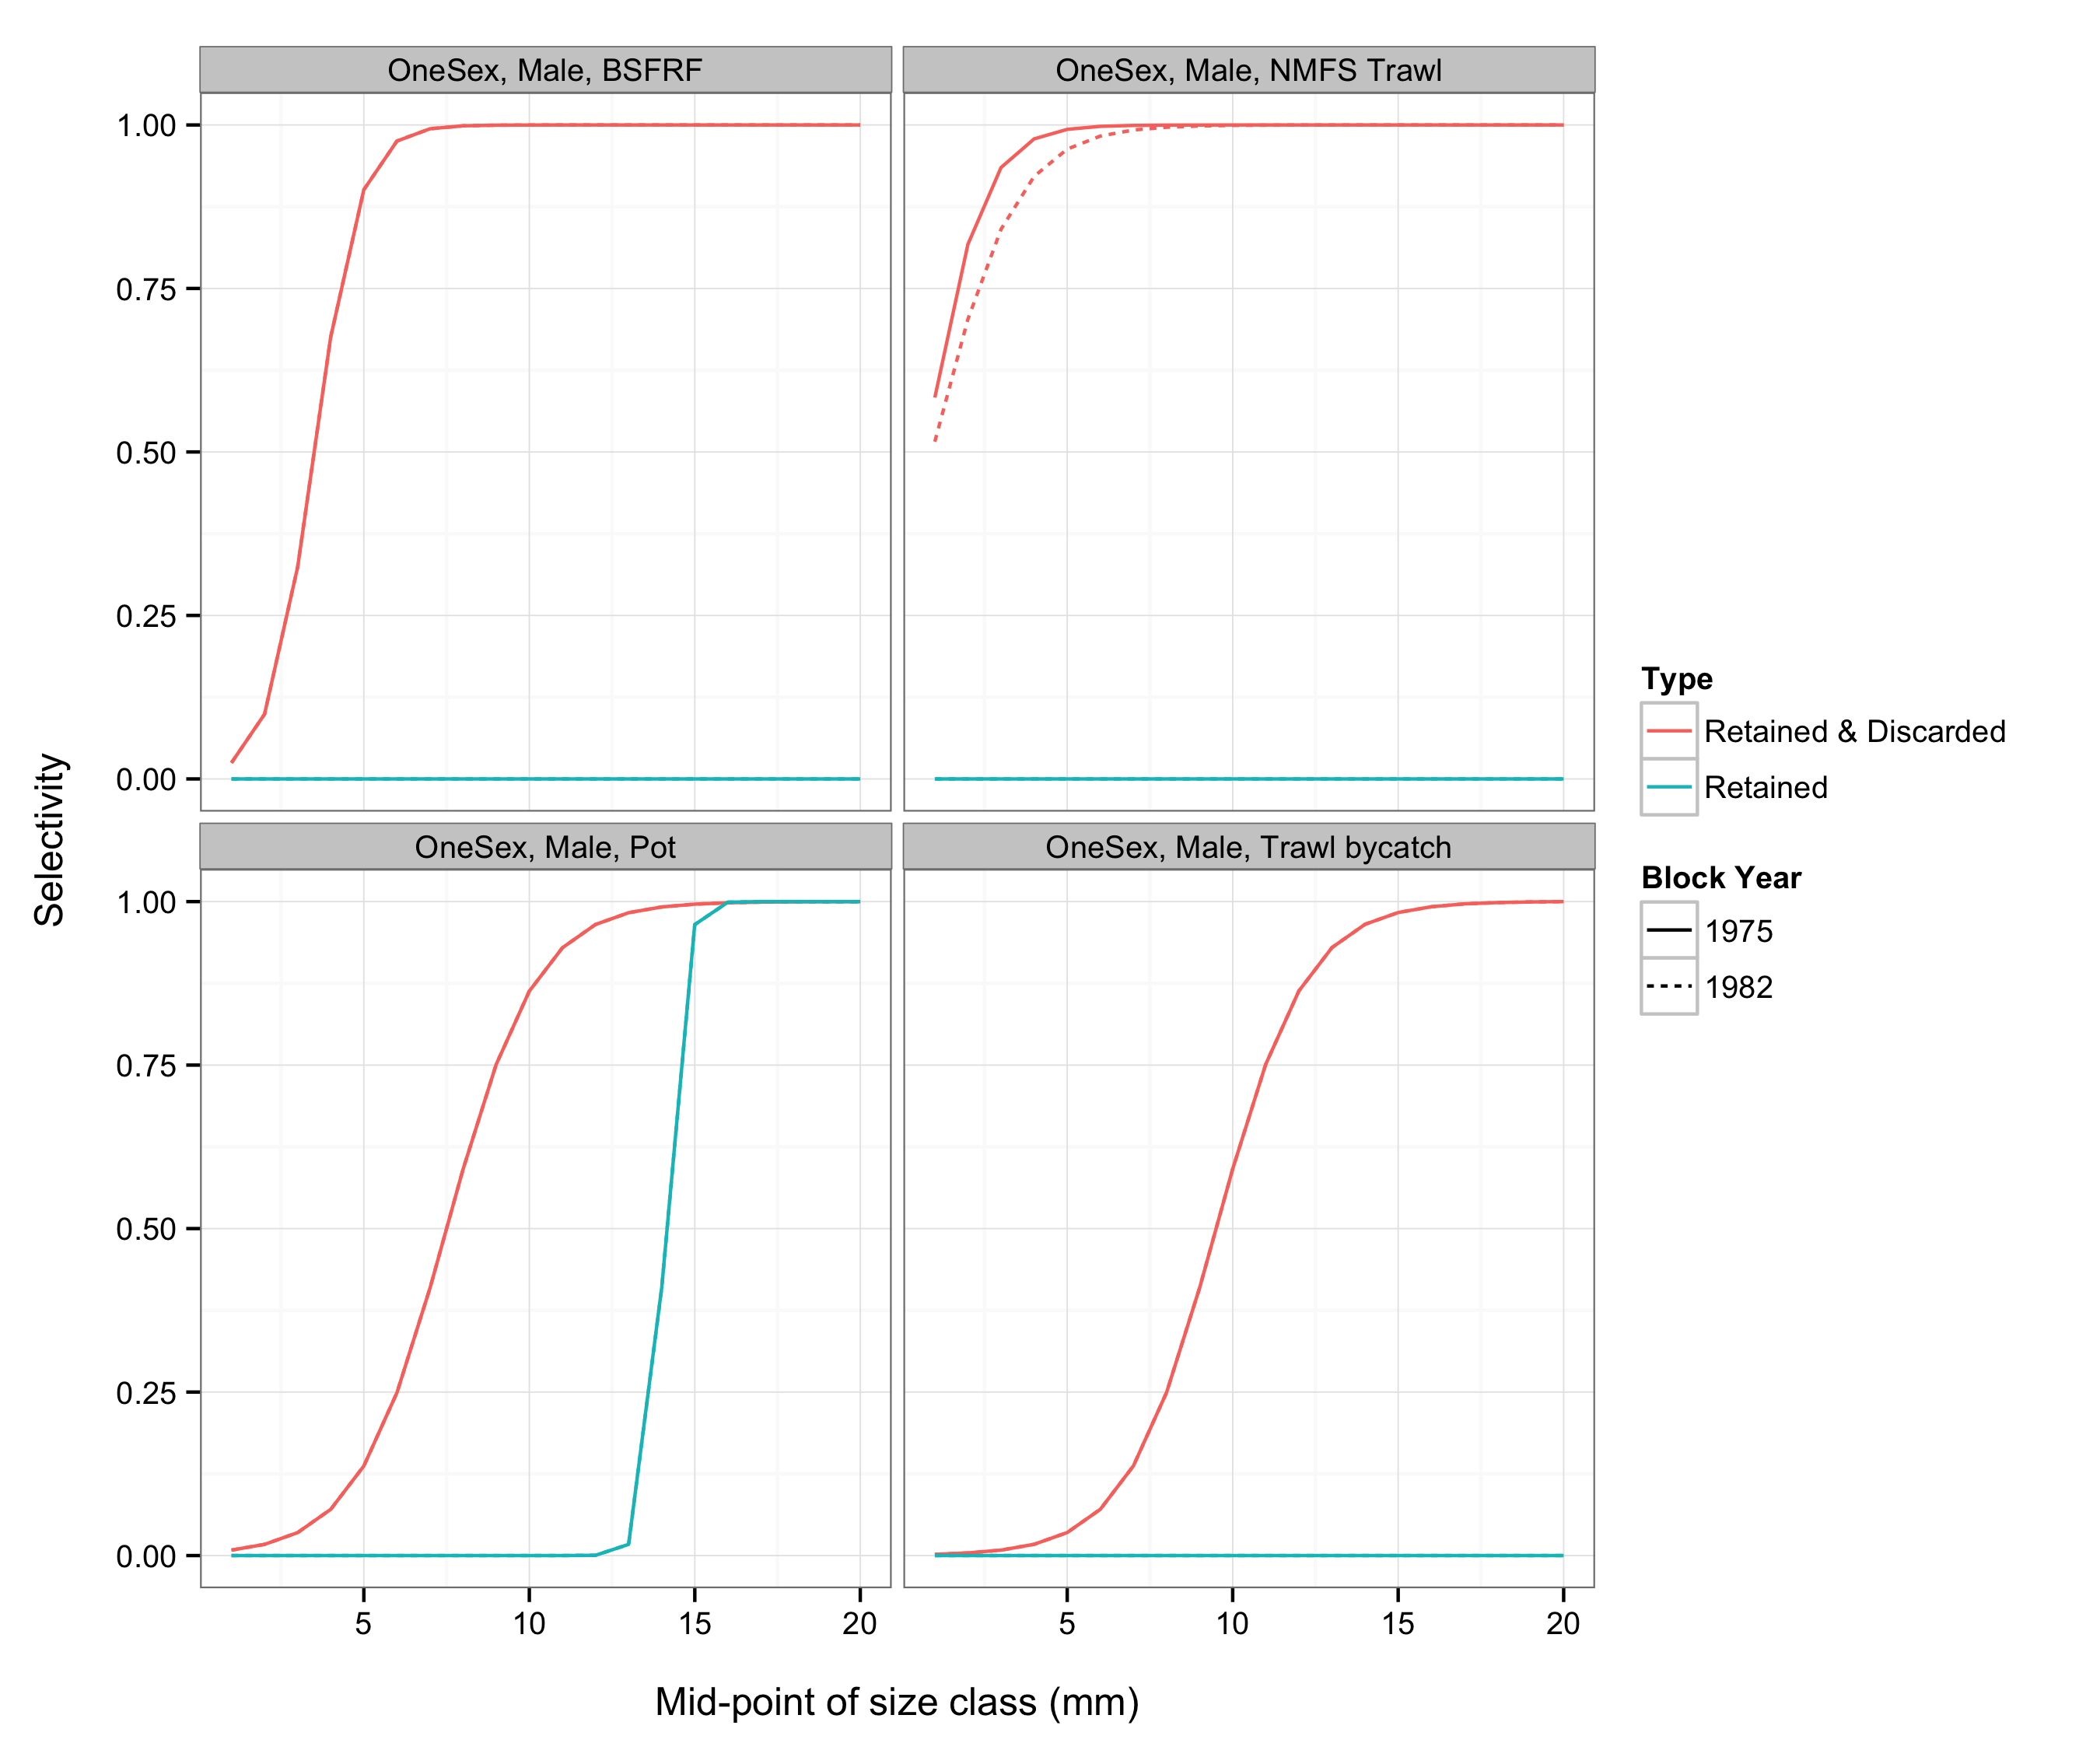
\includegraphics[width=0.6\linewidth]{../../examples/bbrkc/OneSex/figure/selectivity.png}
\end{figure}
\end{frame}

%% =========================================================================== %%

\begin{frame}
\frametitle{Fishing mortality}
\begin{align*}
  \boldsymbol{F}_{h,i} &= \sum_k \exp \left( \bar{\boldsymbol{f}}_k +
    \boldsymbol\Psi_{k,i} \right) \boldsymbol\nu_{h,i,k},\\
\end{align*}

\begin{equation*}
  C_{h,i} = \sum_{\ell} \left[ \boldsymbol{n}_{h,i} \boldsymbol{w}_{h} \frac{\boldsymbol{F}_{h,i}}{\boldsymbol{Z}_{h,i}} 
    \left( 1 - e^{-\boldsymbol{Z}_{h,i}} \right) \right] \quad \text{where} \quad \boldsymbol{Z}_{h,i}
  = M_{h,i} + \boldsymbol{F}_{h,i}.
\end{equation*}

\end{frame}

%% =========================================================================== %%
%% =========================================================================== %%

\section{Natural mortality and survival}

%% =========================================================================== %%
%% =========================================================================== %%

\subsection{Natural mortality}
\begin{frame}
\frametitle{Natural mortality}
\begin{table}
  \centering
  \begin{tabular}{cl}
  \hline
  Symbol  & Description \\
  \hline
      $\textcolor{red}{M_{0,h}}$ &  \\
      $\sigma_M$ & Standard deviation of natural mortality \\
      $\delta_i$ & Natural mortality deviate \\
      $M_{h,i}$ & Natural mortality by sex $h$ and year $i$ \\
  \hline
  \end{tabular}
\end{table}
\end{frame}

%% =========================================================================== %%

\begin{frame}
\frametitle{Natural mortality options}
Natural mortality ($M$) is assumed to be sex-specific ($h$), size-independent
($\ell$), and may or may not be constant over time ($i$). The options currently
available in Gmacs include:
\begin{enumerate}
\item Constant natural mortality ($M_{h,i} = \textcolor{red}{M_{0,h}}$)
\item Random walk (deviates constrained by variance $\sigma^2_M$)
\item Cubic Spline (deviates constrained by nodes and node placement)
\item Blocked changes (deviates constrained by variance at specific knots)
\end{enumerate}
\end{frame}

%% =========================================================================== %%

\begin{frame}
\frametitle{Natural mortality: option 2}
If time-varying natural mortality is specified using the {\bf random walk}
option, the model constrains $M_{h,i}$ to be a random-walk process with variance
$\sigma^2_M$
\begin{equation*}
  M_{h,i+1} = 
  \begin{cases}
    \textcolor{red}{M_{0,h}} \\
    M_{h,i} e^{\delta_i}
  \end{cases},
\end{equation*}
where
\begin{equation*}
  \delta_i \sim \mathcal{N} \left( 0, \sigma^2_M \right).
\end{equation*}
A time-varying natural mortality can be estimated for all years ($i$), or for
specified blocks of years ($\iota \in i$).
\begin{figure}[!htbp]
  \centering
  %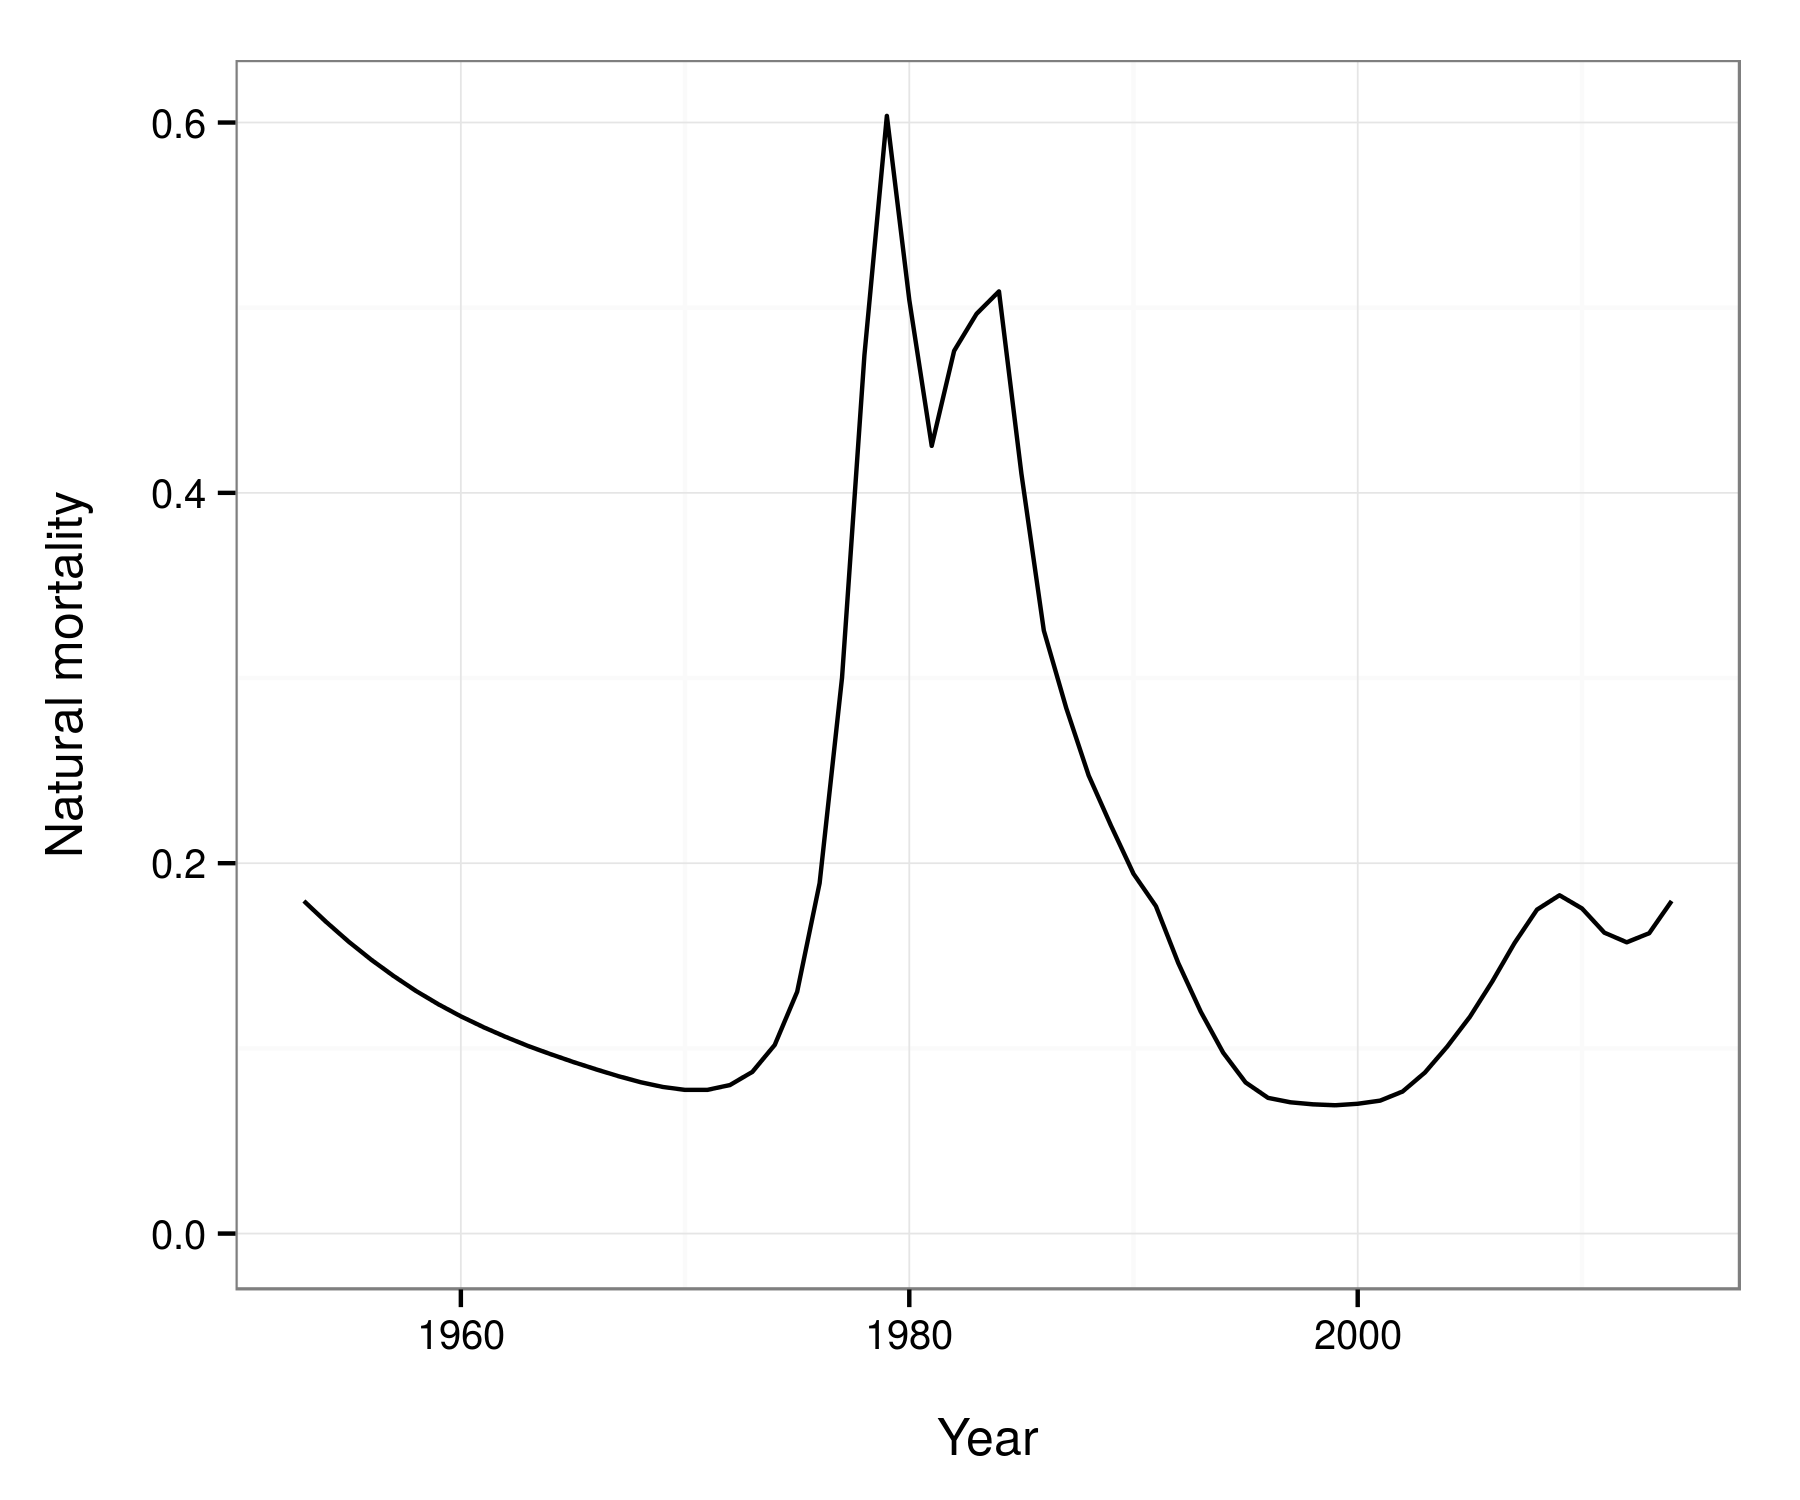
\includegraphics[width=0.65\linewidth]{figure/M_t_walk.png}
\end{figure}
\end{frame}

%% =========================================================================== %%

\begin{frame}
\frametitle{Natural mortality: option 3}
If time-varying natural mortality is specified using the {\bf cubic spline}
option, the model constrains $M_{h,i}$ to be a cubic spline process at
specified knots. For example, setting
\begin{figure}[!htbp]
  \centering
  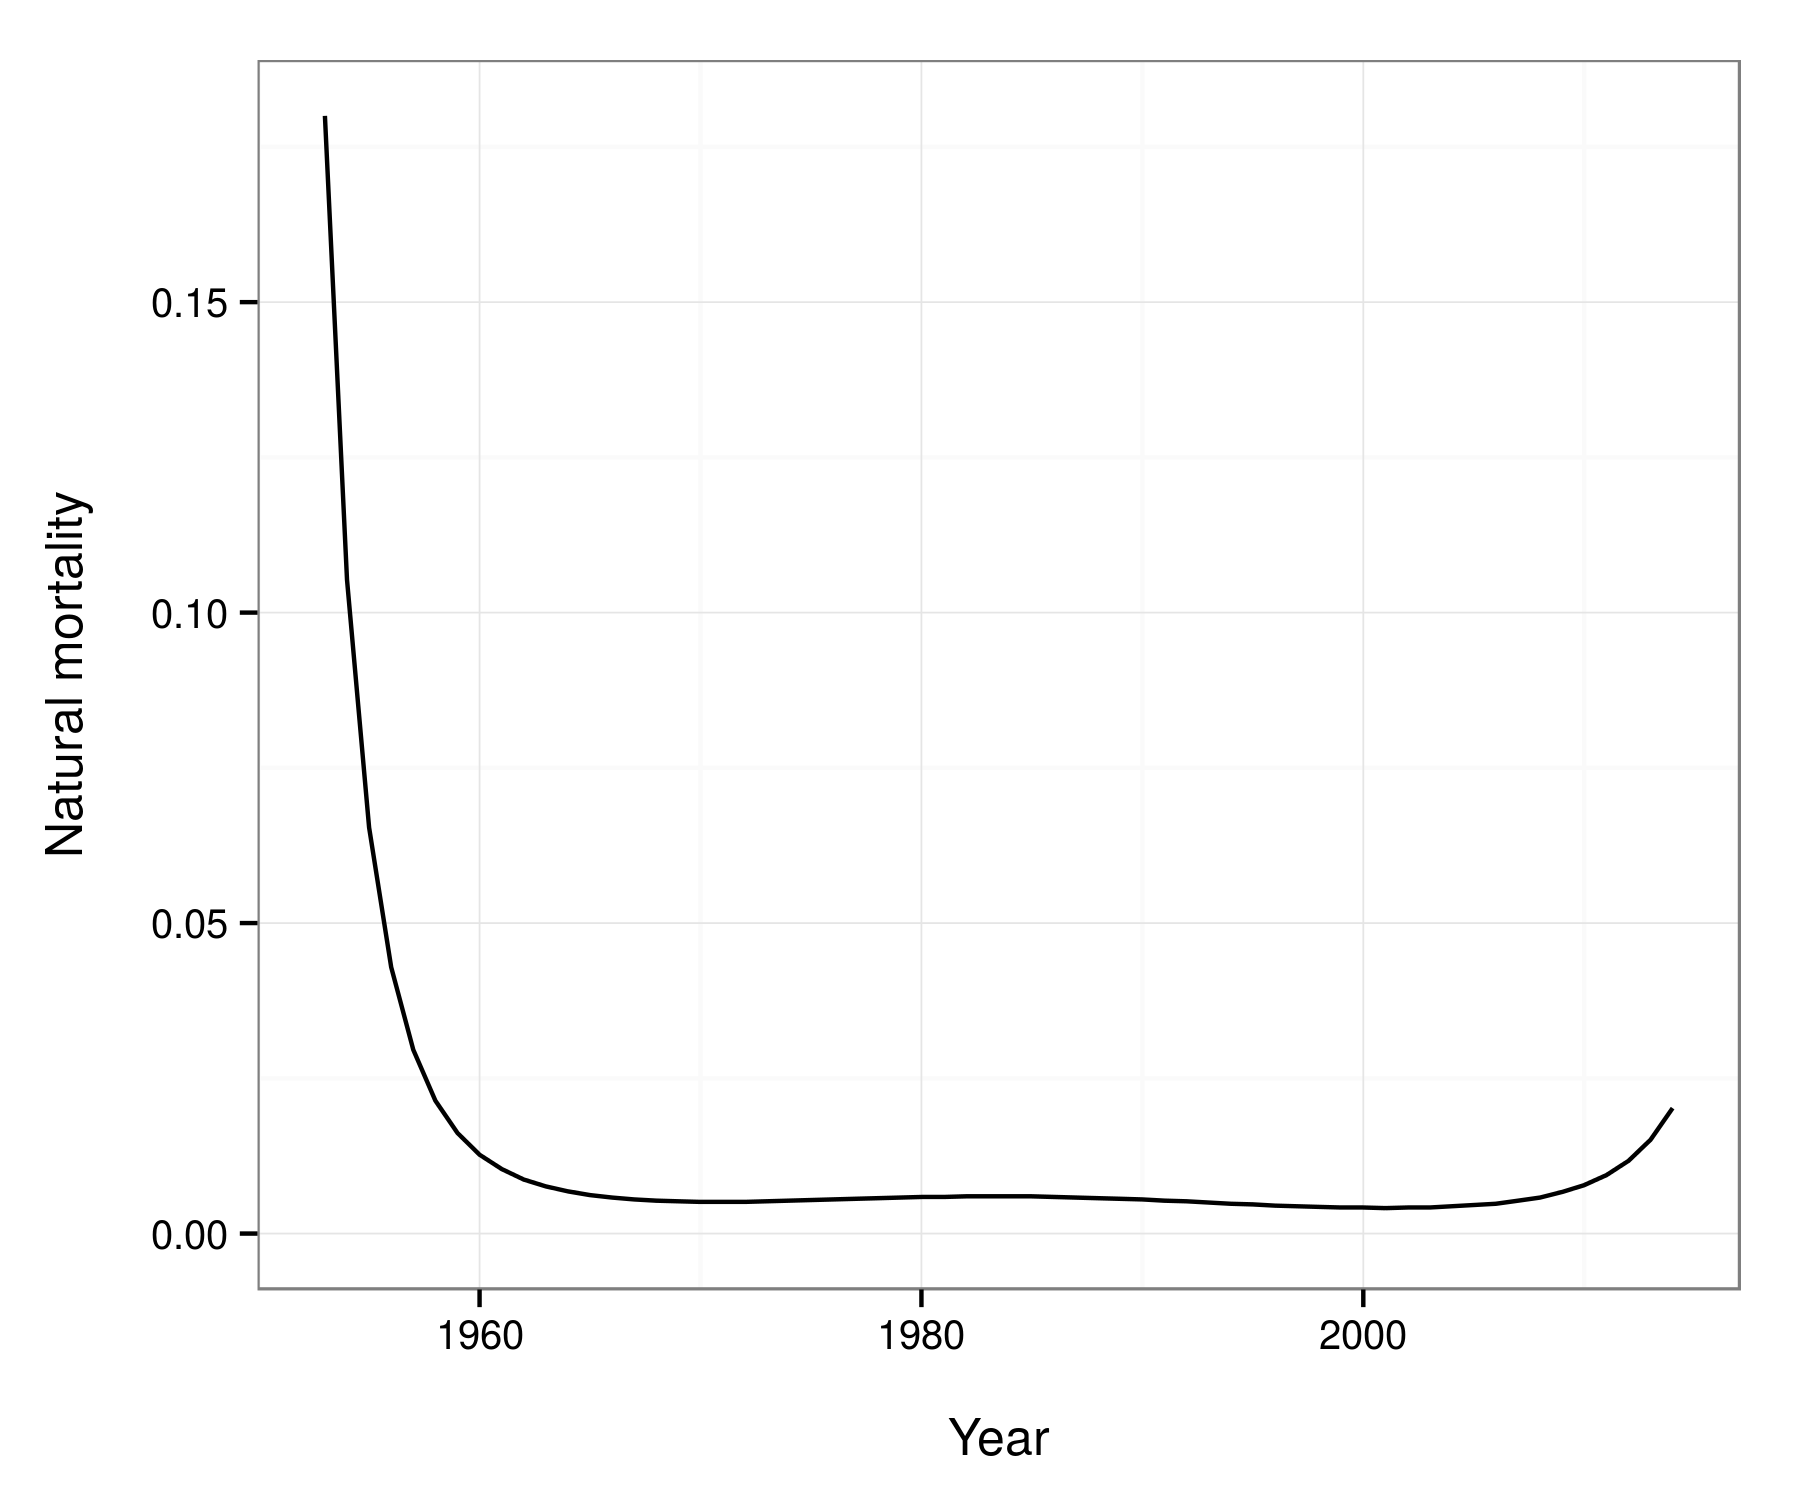
\includegraphics[width=0.65\linewidth]{figure/M_t_spline.png}
\end{figure}
\end{frame}

%% =========================================================================== %%

\begin{frame}
\frametitle{Natural mortality: option 4}
If time-varying natural mortality is specified using the {\bf blocked changes}
option, the model constrains $M_{h,i}$ by the variance ($\sigma^2_M$). For
example, setting $\sigma^2_M = 0.04$ and four specific years (1976, 1980, 1985,
1994) we get
\begin{figure}[!htbp]
  \centering
  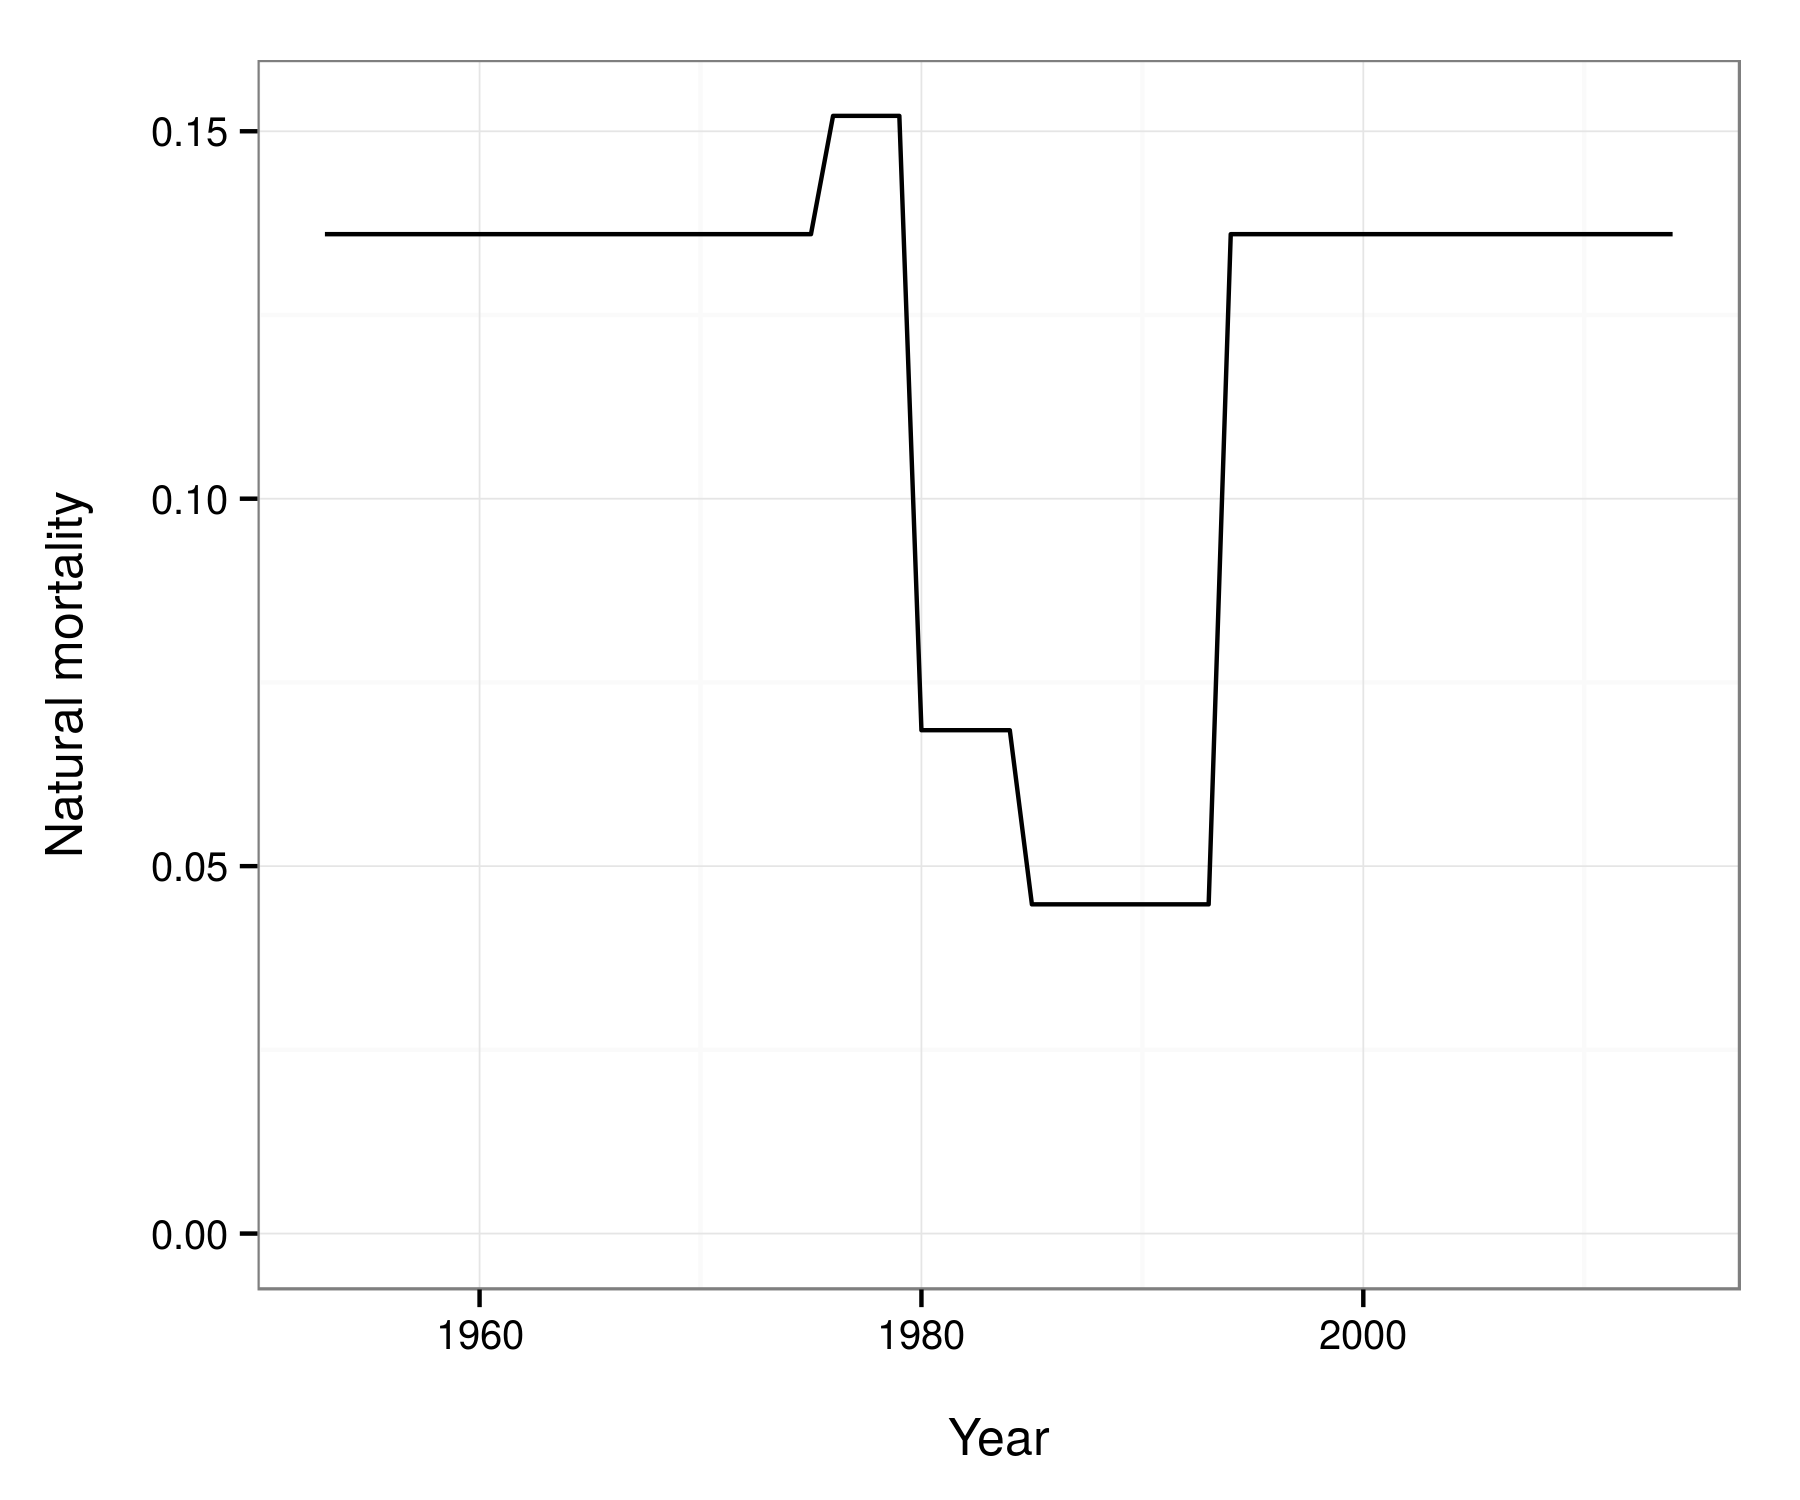
\includegraphics[width=0.65\linewidth]{figure/M_t_block.png}
\end{figure}
\end{frame}

%% =========================================================================== %%
%% =========================================================================== %%

\section{Recruitment}

%% =========================================================================== %%
%% =========================================================================== %%

\begin{frame}
\frametitle{Recruitment}
Recruitment size-distribution
\begin{align*}
  \alpha &= \frac{\alpha_r}{\beta_r},\\
  p(\boldsymbol{r}_i) &= \int^{x_\ell+0.5 \Delta x}_{x_\ell-0.5 \Delta x}
  \frac{x^{\alpha-1} \exp
    \left(\frac{x}{\beta_r}\right)}{\Gamma (\alpha) x^\alpha} dx,\\
  \boldsymbol{r}_{h,i} &= 0.5 p(\boldsymbol{r}_i) \ddot{R}.
\end{align*}
\end{frame}

%% =========================================================================== %%
%% =========================================================================== %%

\section{Initialization}

%% =========================================================================== %%
%% =========================================================================== %%

\subsection{Initialization}
\begin{frame}
\frametitle{Initialization}
Growth and survival
\begin{equation*}
  \boldsymbol{A}_{h} = \boldsymbol{G}_h \left[ \exp (-\textcolor{red}{M_{0,h}})
    \boldsymbol{I} \right] \quad \text{for} \quad i=1.
\end{equation*}

\begin{equation*}
  \boldsymbol{u}_h = -(\boldsymbol{A}_h - \boldsymbol{I})^{-1} (p[\boldsymbol{r}]),
\end{equation*}

Steady-state conditions
\begin{equation*}
  B_0 = \textcolor{red}{R_0} \sum_h \lambda_h \sum_\ell \boldsymbol{u}_h
  \boldsymbol{w}_{h} \boldsymbol{m}_{h},
\end{equation*}
The total unfished numbers in each size category is defined as $R_0
\boldsymbol{u}_h$. Initial numbers at length
\begin{equation*}
  \boldsymbol{n}_{h,i} = \left[-\left( \boldsymbol{A}_{h} - \boldsymbol{I}
    \right)^{-1} \boldsymbol{r}_{h,i} \right] e^{\boldsymbol\nu} \quad
  \text{where} \quad i=1.
\end{equation*}
\end{frame}

%% =========================================================================== %%



%% =========================================================================== %%
%% =========================================================================== %%

\section{Steady-state conditions}

%% =========================================================================== %%
%% =========================================================================== %%

\subsection{Survivorship to length}
\begin{frame}
\frametitle{Survivorship to length}
Assuming a non-zero steady-state fishing mortality rate vector
$\boldsymbol{f}_{h,i}$, the equilibrium growth and survival process is
represented by
\begin{equation*}
  \boldsymbol{B}_{h,i} = \boldsymbol{G}_h \left[ \exp (-M_{h,i} -
    \boldsymbol{f}_{h,i}) \boldsymbol{I} \right].
\end{equation*}
The vector $\boldsymbol{f}_{h,i}$ represents all mortality associated with
fishing, including discards in directed and non-directed fisheries.

Assuming unit recruitment, then the growth and survivorship in unfished and
fished conditions is given by the solutions to the matrix equations
\begin{equation*}
  \boldsymbol{v}_h = -(\boldsymbol{B}_h - \boldsymbol{I})^{-1} (p[\boldsymbol{r}]).
\end{equation*}
The vector $\boldsymbol{v}_h$ represent the unique equilibrium solution for the
numbers per recruit in each size category.

\begin{equation*}
  \tilde{B} = \tilde{R} \sum_h \lambda_h \sum_\ell \boldsymbol{v}_h \boldsymbol{w}_{h}
  \boldsymbol{m}_{h}.
\end{equation*}
\end{frame}

%% =========================================================================== %%

\begin{frame}
\frametitle{Population dynamics}
The numbers in each size-class in the following time-step
($\boldsymbol{n}_{h,i+1}$) is the product of the numbers in each size-class in
the previous time-step ($\boldsymbol{n}_{h,i}$), size-specific growth and
survival ($\boldsymbol{B}_{h,i}$), plus new recruits ($\boldsymbol{r}_{h,i}$)
\begin{equation*}
  \boldsymbol{n}_{h,i+1} = \boldsymbol{n}_{h,i} \boldsymbol{B}_{h,i} +
  \boldsymbol{r}_{h,i} \quad \text{where} \quad i > 1.
\end{equation*}
\end{frame}

%% =========================================================================== %%
%% =========================================================================== %%

\section{Likelihoods}

%% =========================================================================== %%
%% =========================================================================== %%

\subsection{Log-likelihoods}
\begin{frame}
\frametitle{Log-likelihoods}
In general, if we have a random variable $x$ that is normally distributed with
mean $\mu$ and variance $\sigma^2$, we write
\begin{equation*}
  x \sim \mathcal{N} \left(\mu, \sigma^2 \right).
\end{equation*}
The log-likelihood is
\begin{equation*}
  \ell(\mu,\sigma^2; x_1,\ldots,x_n) = \cancel{-\frac{n}{2} \log (2 \pi)} - n \log (\sigma) -
  \frac{1}{2\sigma^2} \sum_i^n (x_i - \mu)^2.
\end{equation*}
If a coefficient of variation $c$ is defined, rather than a standard deviation
$\sigma$ we write
\begin{equation*}
  \sigma = \sqrt{\log \left( 1+c^2 \right)}.
\end{equation*}


If we have a random variable $x$ that is log-normally distributed with
location $\mu$ and scale $\sigma$, we write
\begin{equation*}
  x \sim \log \mathcal{N} \left(\mu, \sigma^2 \right).
\end{equation*}
The log-likelihood is
\begin{equation*}
  \ell(\mu,\sigma^2; x_1,\ldots,x_n) = -\frac{n}{2} \log (2 \pi) - n \log (\sigma) -
  \frac{1}{2\sigma^2} \sum_i^n (x_i - \mu)^2.
\end{equation*}
\end{frame}

%% =========================================================================== %%

\begin{frame}
\frametitle{Log-likelihoods: catch}
The standard deviation is calculated from the CV as
\begin{equation*}
  \sigma = \sqrt{\log \left( 1+c^2 \right)}.
\end{equation*}
The log-likelihood is
\begin{equation*}
  \ell(\mu,\sigma^2; x_1,\ldots,x_n) = \cancel{-\frac{n}{2} \log (2 \pi)} - n \log (\sigma) -
  \frac{1}{2\sigma^2} \sum_i^n (x_i - \mu)^2.
\end{equation*}
\end{frame}

%% =========================================================================== %%

\begin{frame}
\frametitle{Log-likelihoods: relative abundance}
the catchability coefficient $q$ is treated as a nuisance parameter and
integrated out of the model (Walters and Ludwig 1994)
\begin{equation*}
  q = \exp \left( \frac{1}{n} \sum_i \log \left( \frac{I_i}{V_i} \right) \right).
\end{equation*}

\begin{equation*}
  I_i = q V_i
\end{equation*}
The standard deviation is calculated from the CV as
\begin{equation*}
  \sigma = \sqrt{\log \left( 1+c^2 \right)}.
\end{equation*}
The log-likelihood is
\begin{align*}
  \ell(\mu,\sigma^2; x_1,\ldots,x_n)
  &= n \lambda \cancel{-\frac{n}{2} \log (2 \pi)} - n \log (\sigma) - \frac{1}{2\sigma^2} \sum_i^n (x_i - \mu)^2\\
  &= n \lambda - n \log (\sigma) - \frac{1}{2\sigma^2} \sum_i^n (x_i - \mu)^2\\
\end{align*}
\end{frame}

%% =========================================================================== %%

\begin{frame}
\frametitle{Log-likelihoods}
Fishing mortality
\begin{equation*}
  \ell(F_k) = 0.5 \log (2 \pi) + \log (\sigma_{F_k}) + 0.5
  \frac{1}{\sigma^2_{F_k}} (\bar{F}_k - \hat{F})^2.
\end{equation*}
Natural mortality
\begin{equation*}
  \ell(M_h) = 
  \begin{cases}
    0.5 \log (2 \pi) + \log (\sigma_{M_h}) + 0.5 \frac{1}{\sigma^2_{M_h}} \sum_i
    \delta_i^2 \quad \text{or}\\
    0.5 \log (2 \pi) + \log (\sigma_{M_h}) + 0.5 \frac{1}{\sigma^2_{M_h}} \sum_i
    (\delta_{i+1} - \delta_i)^2
  \end{cases}.
\end{equation*}
Abundance indices
\begin{equation*}
  \ell(I_k) = 0.5 \log (2 \pi) + \log (\sigma_{F_k}) + 0.5
  \frac{1}{\sigma^2_{F_k}} (\bar{F}_k - \hat{F})^2.
\end{equation*}

\end{frame}

%% =========================================================================== %%

\begin{frame}
\frametitle{Data weighting}
Log-likelihood, likelihood, distribution
\begin{align*}
  \ell (\mu, \sigma^2, \lambda; x) &= \lambda \left( -\frac{1}{2} \log (2 \pi) - \frac{1}{2}
  \log (\sigma^2) - \frac{1}{2 \sigma^2} (x - \mu)^2 \right)\\
  p(x|\mu, \sigma^2, \lambda) &= \exp(\lambda) \left( 2 \pi \sigma^2 \right)^{-\frac{1}{2}} \exp \left[ -\frac{1}{2
      \sigma^2} (x - \mu)^2 \right]\\
  x|\mu, \sigma^2, \lambda &\sim \mathcal{N} \left( \mu, \lambda \sigma^2 \right)
\end{align*}
\end{frame}

%% =========================================================================== %%

\end{document}